\documentclass[10pt,pdf,hyperref={unicode},aspectratio={169}]{beamer}
\usepackage{lmodern}
\usepackage[T2A]{fontenc}
\usepackage[utf8]{inputenc}
\usepackage{graphicx}
\usepackage{amsmath}

\DeclareGraphicsRule{.gif}{eps}{.gif.bb}{‘convert #1 ’eps:-’ }

% отключить клавиши навигации
% \setbeamertemplate{navigation symbols}{}
% тема оформления
\usetheme{default}
% цветовая схема
\usecolortheme{dove}

\title{Моделирование деградации процессов записи/удаления в энергонезависимой памяти на основе квантовых точек}

\author[Прохоров М.Д.]{Выполнил: студент гр. РЛ6--82 Прохоров М.Д.\\ Руководитель: к.т.н. доц. Данилов И.И}
\date{Москва, 2017}
\institute[BMSTU]{МГТУ им. Н.Э.Баумана}

\begin{document}

\begin{frame}
	\titlepage
\end{frame} 

% \begin{frame}
% 	\tableofcontents
% \end{frame} 
\section{Постановка проблемы}
\begin{frame}
	\frametitle{Постановка проблемы}
	\begin{columns}
	\column{0.6\textwidth}
		\begin{center}
			\includegraphics[width=\textwidth]{assets/DiplomaTrouble1}
		\end{center}
	\column{0.4\textwidth}
		\begin{center}
			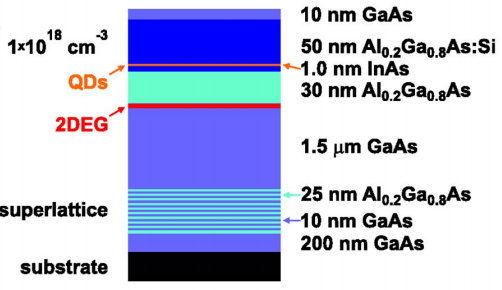
\includegraphics[width=\textwidth]{assets/Flash}
		\end{center}
	\end{columns}
\end{frame}
\begin{frame}
	\frametitle{Постановка проблемы}
	\begin{center}
		\includegraphics[width=0.9\textwidth]{assets/DiplomaTrouble2}
	\end{center}
	Необходимо разработать алгоритм расчета деградации основных параметров QD-Flash для обеспечения заданного уровня надежности еще на этапе проектирования.
\end{frame}
\begin{frame}
	\frametitle{Цели и задачи}
	Цель работы:
	\begin{itemize}
		\item Нахождение модели деградации процессов записи/стирания информации в запоминающих устройствах на основе квантовых точек.
	\end{itemize}
	Задачи работы:
	\begin{itemize}
		\item Исследования механизма деградации гетероструктуры и математического метода моделирования деградации гетероструктуры;
		\item Исследование устройства работы запоминающего устройства на основе квантовых точек и математической модели моделирования процессов записи/стирания информации;
		\item Разработка алгоритма расчета деградации процессов записи/стирания информации в запоминающем устройстве на основе квантовых точек.
	\end{itemize}
\end{frame}

\begin{frame}
	\frametitle{Деградация зонной структуры}
	\begin{columns}
	\column{0.5\textwidth}
		\begin{center}
			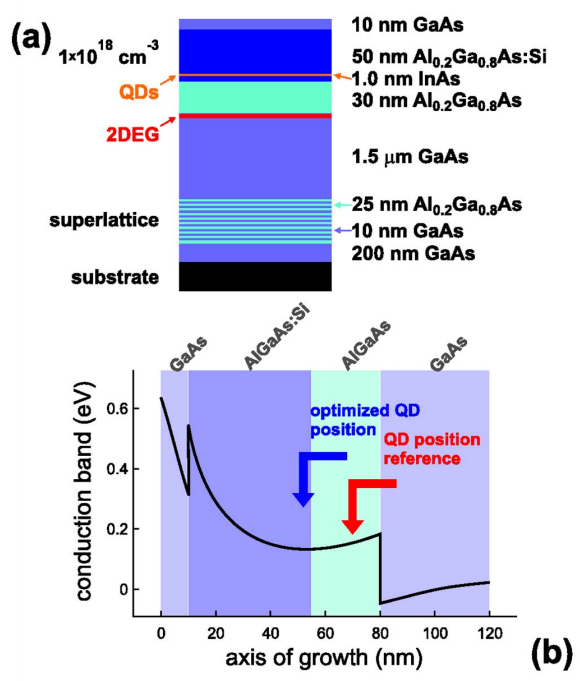
\includegraphics[width=0.9\textwidth]{assets/StuctStructZone}
		\end{center}
	\column{0.5\textwidth}
			Термическая деградации зонной структуры запоминающего устройства обуславливается диффузионным расплытием гетеропереходов:
			\begin{itemize}
				\item $i$--$GaAs$/$n^{+}$--$Al_{x}Ga_{1-x}As$;
				\item $n^{+}$--$Al_{x}Ga_{1-x}As$/$i$--$InAs$;
				\item $i$--$InAs$/$i$--$Al_{y}Ga_{1-y}As$;
				\item $i$--$Al_{y}Ga_{1-y}As$/$i$--$GaAs$.
			\end{itemize}
			Необходимо выяснить какие процессы доминируют, и какими можно пренебречь.
	\end{columns}
\end{frame}

\begin{frame}
	\frametitle{Диффузионное размытие}
	Диффузионное расплытие описывается с законами Фика:
	\begin{gather*}
		\overline{J} = - D \nabla C,\,
		\overline{J}_{x} = - \overline{e}_{x}D_{x} \frac{\delta}{\delta x} C_{x};\\
		\frac{\delta}{\delta t}C = - \nabla (D \nabla C),\,
		\frac{\delta}{\delta t}C_{x} = - \frac{\delta}{\delta x} D_{x} \frac{\delta}{\delta x} C_{x};\\
		D_{i-Al_{x}Ga_{1-x}As} = D_{0}\exp\bigg[-\frac{E_{a}}{k_{B}T}\bigg],\, D_{Al,Si} = D_{i-Al_{x}Ga_{1-x}As}\Big( \frac{N_{D}}{n_{i}} \Big)^{3}.
	\end{gather*}
	Для моделирования диффузионных процессов используются численные методы, одни из них~--- <<Метод конечных разностей>>. Метод заключается в аппроксимации дифференциальных операторов конечными разностями:
	\begin{gather*}
		\frac{\delta y_{i} }{\delta x } = \frac{y_{i+1} - y_{i}}{\Delta x};\\
		\frac{\delta^{2} y_{i} }{\delta x^{2} } = \frac{y_{i+1} - 2y_{i} + y_{i-1}}{\Delta x^2}.
	\end{gather*}
\end{frame}

\begin{frame}
	\frametitle{Конечно-разностная схема для решения II закона Фика, при постоянном коэффициенте диффузии}
	\begin{columns}
	\column{0.5\textwidth}
		<<Закрытая>> система:
		\begin{equation*}
			\begin{cases}
				C^{i+1}_{1} = (1 - \lambda)C^{i}_{1} + \lambda C^{i}_{2};\\
				C^{i+1}_{k} = \lambda C^{i}_{k-1} + (1 - 2\lambda)C^{i}_{k} + \lambda C^{i}_{k+1};\\
				k \in [2,\,\dots,\,N-1];\\
				C^{i+1}_{N} = (1 - \lambda)C^{i}_{N} + \lambda C^{i}_{N-1};\\
				\lambda = D\frac{\Delta t}{\Delta x^{2}}.
			\end{cases}
		\end{equation*}
	\column{0.5\textwidth}
		<<Открытая>> система:
		\begin{equation*}
			\begin{cases}
				C^{i+1}_{1} = C^{i}_{1};\\
				C^{i+1}_{k} = \lambda C^{i}_{k-1} + (1 - 2\lambda)C^{i}_{k} + \lambda C^{i}_{k+1};\\
				k \in [2,\,\dots,\,N-1];\\
				C^{i+1}_{N} = C^{i}_{N};\\
				\lambda = D\frac{\Delta t}{\Delta x^{2}}.
			\end{cases}
		\end{equation*}
	\end{columns}
\end{frame}

\begin{frame}
	\frametitle{Конечно-разностная схема для решения II закона Фика, при коэффициенте диффузии зависящем от концентрации}
	\begin{columns}
	\column{0.5\textwidth}
		<<Закрытая>> система:
		\begin{equation*}
			\begin{cases}
				C^{i+1}_{1} = (1 - \lambda_{+})C^{i}_{1} + \lambda_{+} C^{i}_{2};\\
				C^{i+1}_{k} = \lambda_{-}^{i} C^{i}_{k-1} + (1 - \lambda^{i}_{+} - \lambda^{i}_{-})C^{i}_{k} + \lambda^{i}_{+} C^{i}_{k+1},\\
				k \in [2,\,\dots,\,N-1];\\
				C^{i+1}_{N} = (1 - \lambda_{-})C^{i}_{N} + \lambda_{-} C^{i}_{N-1};\\
				\lambda^{i}_{+} = D_{j+}^{i}\frac{\Delta t}{\Delta x^{2}};\\
				\lambda^{i}_{-} = D_{j-}^{i}\frac{\Delta t}{\Delta x^{2}};\\
				D_{j\pm}^{i} = \frac{D^{i}_{j} + D^{i}_{j\pm1}}{2}.
			\end{cases}
		\end{equation*}
	\column{0.5\textwidth}
		<<Открытая>> система:
		\begin{equation*}
			\begin{cases}
				C^{i+1}_{1} = C^{i}_{1};\\
				C^{i+1}_{k} = \lambda_{-}^{i} C^{i}_{k-1} + (1 - \lambda^{i}_{+} - \lambda^{i}_{-})C^{i}_{k} + \lambda^{i}_{+} C^{i}_{k+1};\\
				k \in [2,\,\dots,\,N-1];\\
				C^{i+1}_{N} = C^{i}_{N};\\
				\lambda^{i}_{+} = D_{j+}^{i}\frac{\Delta t}{\Delta x^{2}};\\
				\lambda^{i}_{-} = D_{j-}^{i}\frac{\Delta t}{\Delta x^{2}};\\
				D_{j\pm}^{i} = \frac{D^{i}_{j} + D^{i}_{j\pm1}}{2}.
			\end{cases}
		\end{equation*}
	\end{columns}
\end{frame}

\begin{frame}
	\frametitle{Исследование диффузионного расплытия гетероструктур}
	\begin{columns}
	\column{0.6\textwidth}
		Исследуем расплытие данных гетероструктур:
		\begin{itemize}
			\item $i$--$GaAs$/$n^{+}$--$Al_{x}Ga_{1-x}As$;
			\item $n^{+}$--$Al_{x}Ga_{1-x}As$/$i$--$InAs$;
			\item $i$--$InAs$/$i$--$Al_{y}Ga_{1-y}As$;
			\item $i$--$Al_{y}Ga_{1-y}As$/$i$--$GaAs$.
		\end{itemize}
		на примере симметричной ГС при различных температурах и выявим доминирующий процесс.
	\column{0.4\textwidth}
		Структура для определения доминирующего диффузионного процесса:
		\begin{center}
			\includegraphics[width=0.5\textwidth]{assets/DifCloseAlGaAs3D}
		\end{center}
	\end{columns}
\end{frame}

\begin{frame}
	\frametitle{Моделирование диффузионного размытия $i\!-\!GaAs/i\!-\!Al_{45}Ga_{55}As$}
	\begin{columns}
	\column{0.5\textwidth}
		\begin{center}
			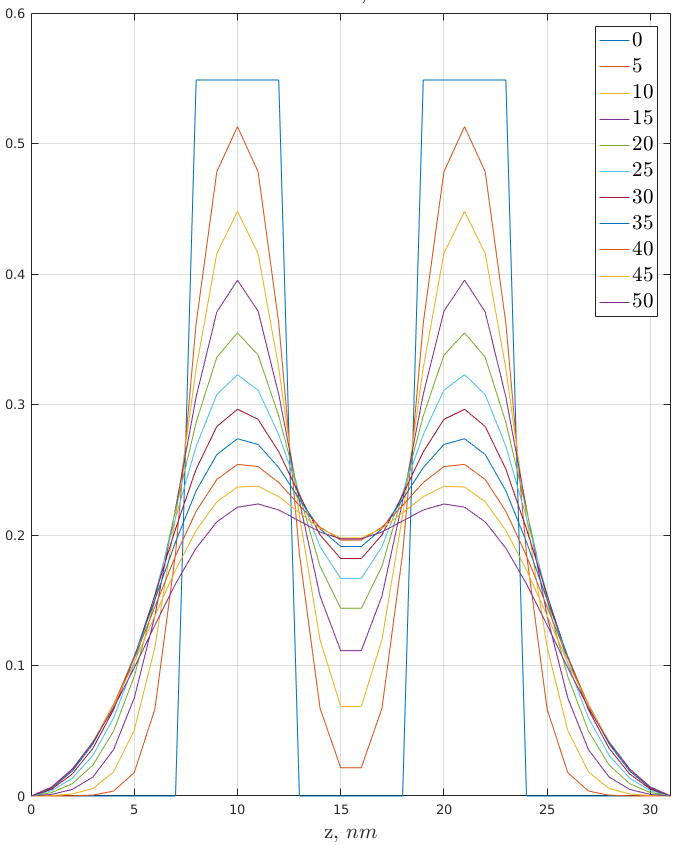
\includegraphics[width=0.75\textwidth]{assets/D1CAlGaAs}
		\end{center}
		<<Закрытая>> система при $T = 800K$.
	\column{0.5\textwidth}
		\begin{center}
			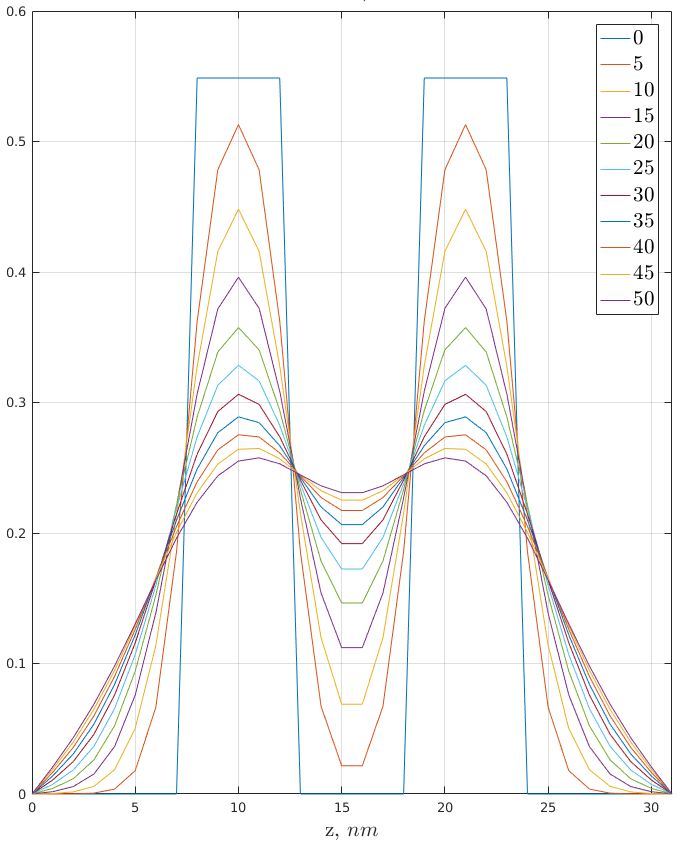
\includegraphics[width=0.75\textwidth]{assets/D1OAlGaAs}
		\end{center}
		<<Открытая>> система при $T = 800K$.
	\end{columns}
\end{frame}

\begin{frame}
	\frametitle{Моделирование диффузионного размытия $n\!-\!GaAs/n\!-\!Al_{45}Ga_{55}As$}
	\begin{columns}
	\column{0.5\textwidth}
		\begin{center}
			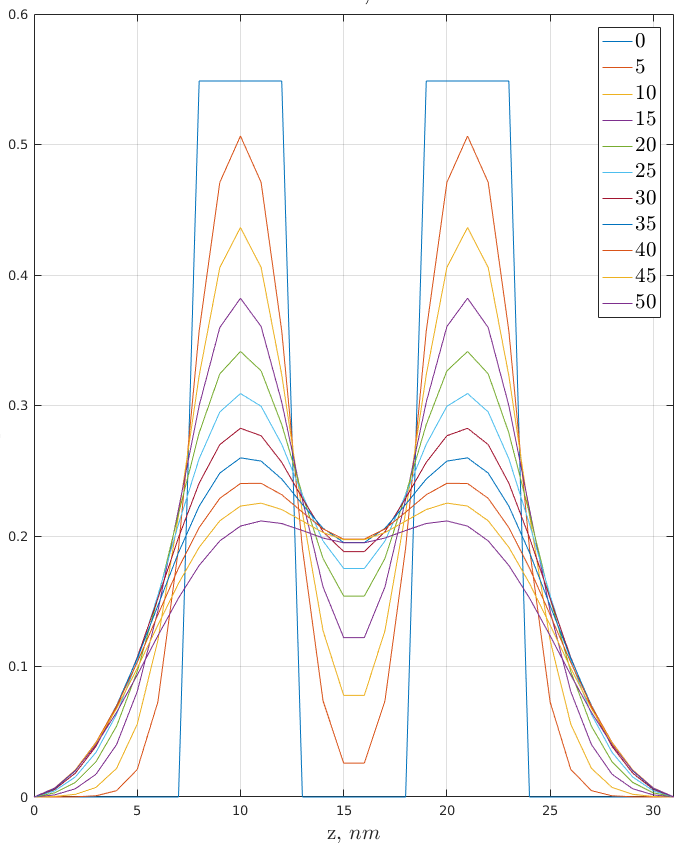
\includegraphics[width=0.75\textwidth]{assets/D1CAlGaAsNd}
		\end{center}
		<<Закрытая>> система при $T = 640K$ и $Nd = 5*10^{15} sm^{-3}$.
	\column{0.5\textwidth}
		\begin{center}
			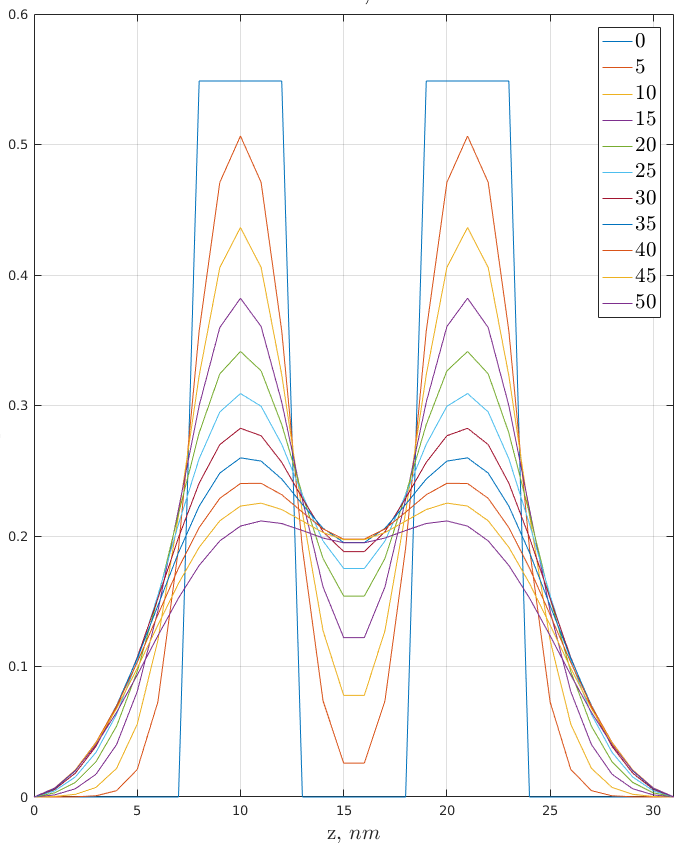
\includegraphics[width=0.75\textwidth]{assets/D1CAlGaAsNd}
		\end{center}
		<<Закрытая>> система при $T = 640K$ и $Nd = 5*10^{15} sm^{-3}$.
	\end{columns}
\end{frame}

\begin{frame}
	\frametitle{Моделирование диффузионного размытия $n^{+}\!-\!GaAs/i\!-\!GaAs/i\!-\!Al_{45}Ga_{55}As/ n^{+}\!-\!GaAs$}
		\begin{center}
			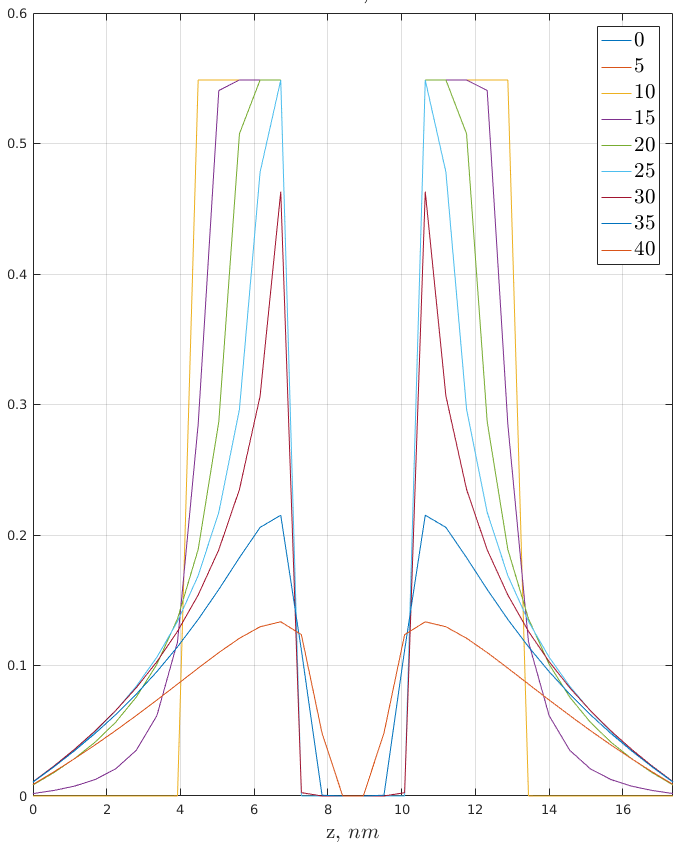
\includegraphics[width=0.38\textwidth]{assets/D1AlGaAs_Si}

			Система при $T = 350K$ и $Nd = 2*10^{17} sm^{-3}$
		\end{center}
\end{frame}

\begin{frame}
	\frametitle{Численный метод моделирования токопереноса через гетероструктуру}
	При моделировании токопереноса через гетероструктуру воспользуемся методом конечных разностей:
\end{frame}

\begin{frame}
	\frametitle{Моделирование моделирование деградации ВАХ ГС $i\!-\!GaAs/i\!-\!Al_{45}Ga_{55}As$}
	\begin{columns}
	\column{0.5\textwidth}
		\begin{center}
			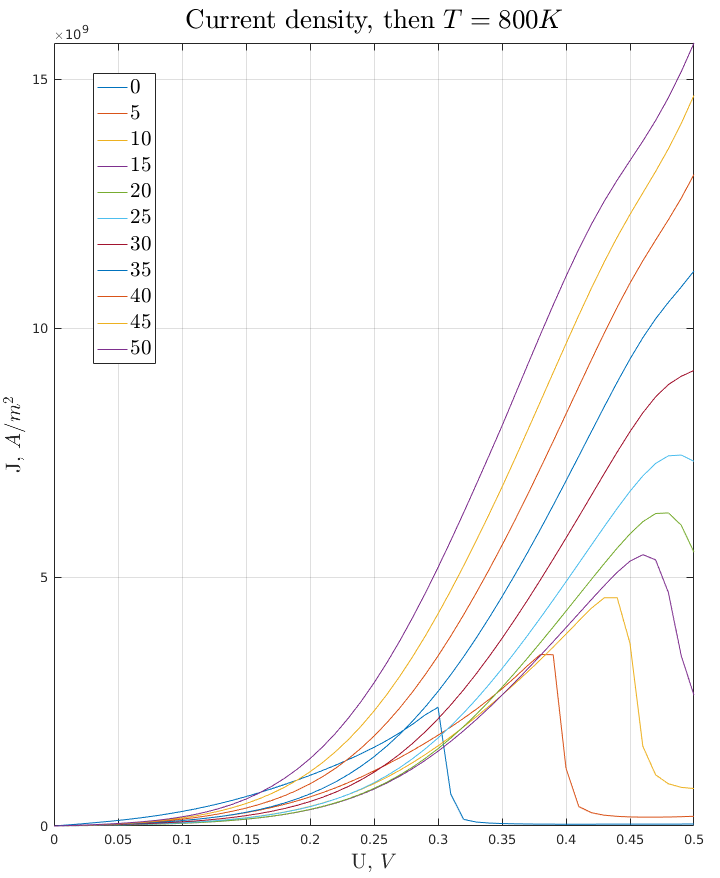
\includegraphics[width=0.7\textwidth]{assets/J1DCAlGaAs}

			<<Закрытая>> система при $T = 800K$.
		\end{center}
	\column{0.5\textwidth}
		\begin{center}
			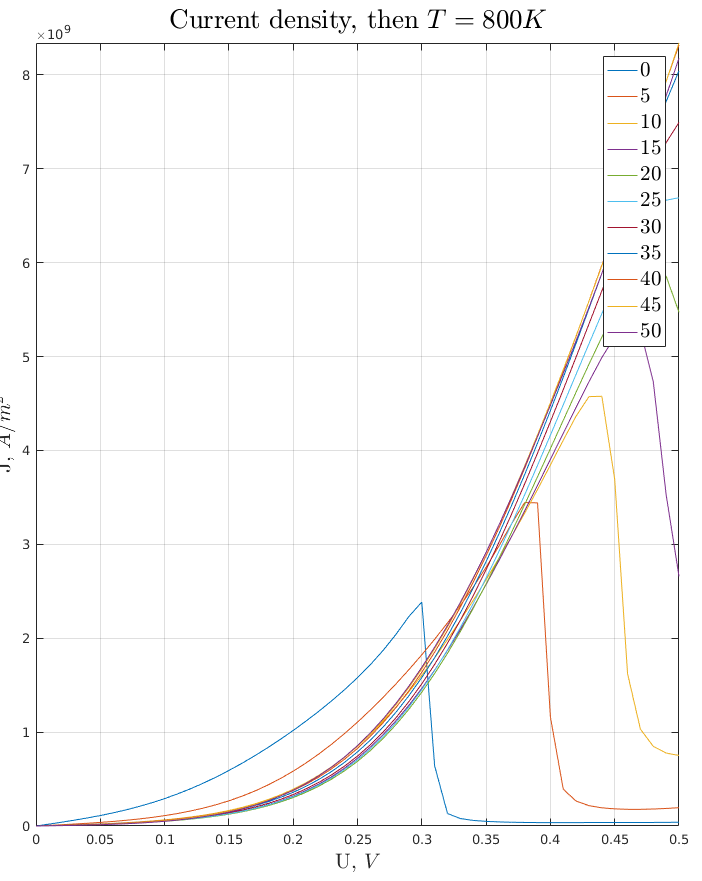
\includegraphics[width=0.7\textwidth]{assets/J1DOAlGaAs}

			<<Открытая>> система при $T = 800K$.
		\end{center}
	\end{columns}
\end{frame}

\begin{frame}
	\frametitle{Моделирование моделирование деградации ВАХ ГС $n\!-\!GaAs/n\!-\!Al_{45}Ga_{55}As$}
	\begin{columns}
	\column{0.5\textwidth}
		\begin{center}
			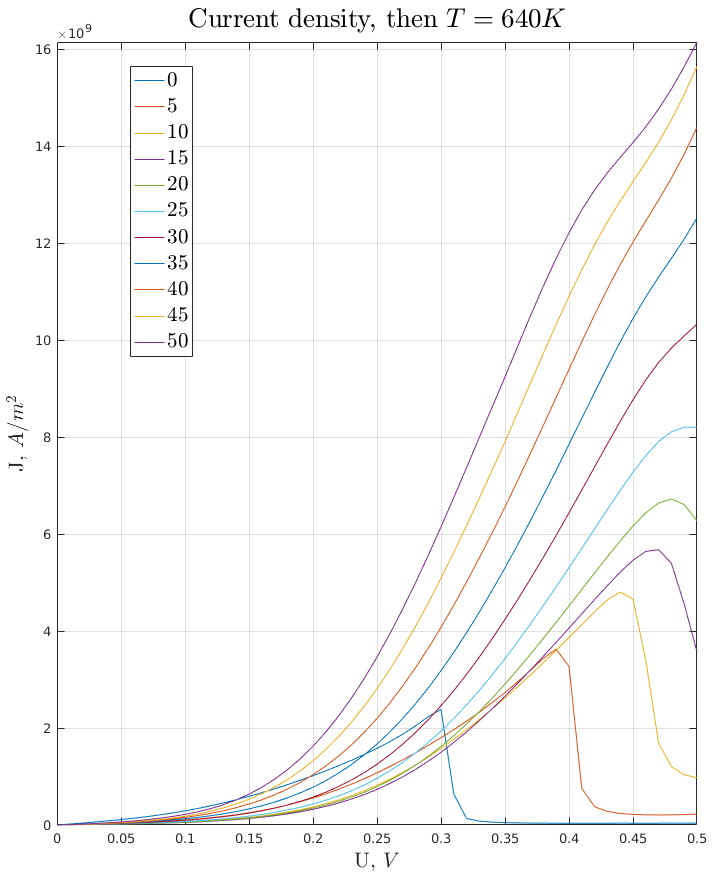
\includegraphics[width=0.7\textwidth]{assets/J1DCAlGaAsNd}

			<<Закрытая>> система при $T = 640K$ и $Nd = 5*10^{15} sm^{-3}$.
		\end{center}
	\column{0.5\textwidth}
		\begin{center}
			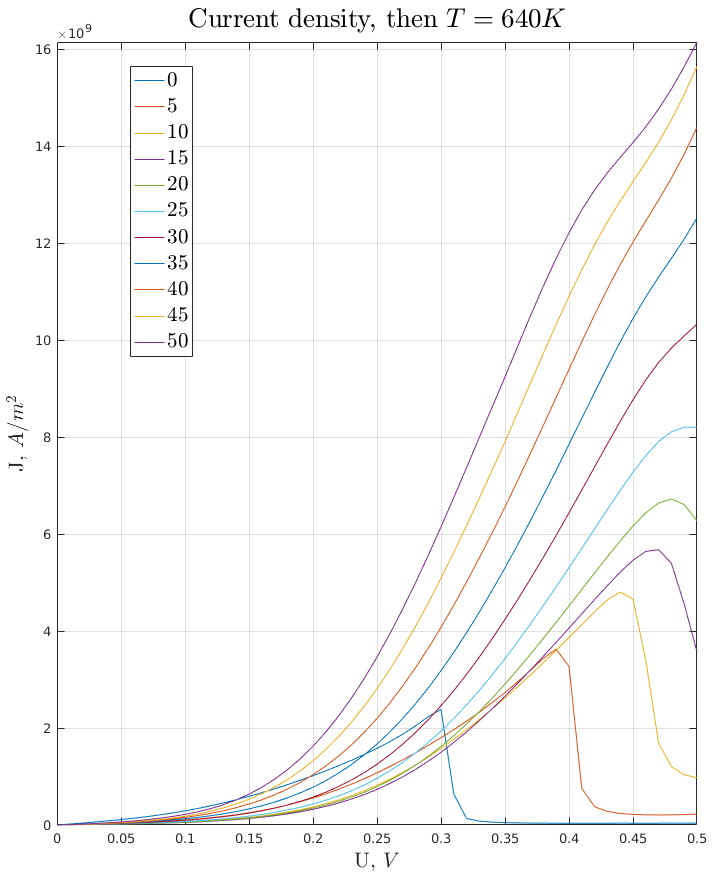
\includegraphics[width=0.7\textwidth]{assets/J1DCAlGaAsNd}

			<<Закрытая>> система при $T = 640K$ и $Nd = 5*10^{15} sm^{-3}$.
		\end{center}
	\end{columns}
\end{frame}

\begin{frame}
	\frametitle{Моделирование моделирование деградации ВАХ ГС $n^{+}\!-\!GaAs/i\!-\!GaAs/i\!-\!Al_{45}Ga_{55}As/ n^{+}\!-\!GaAs$}
		\begin{center}
			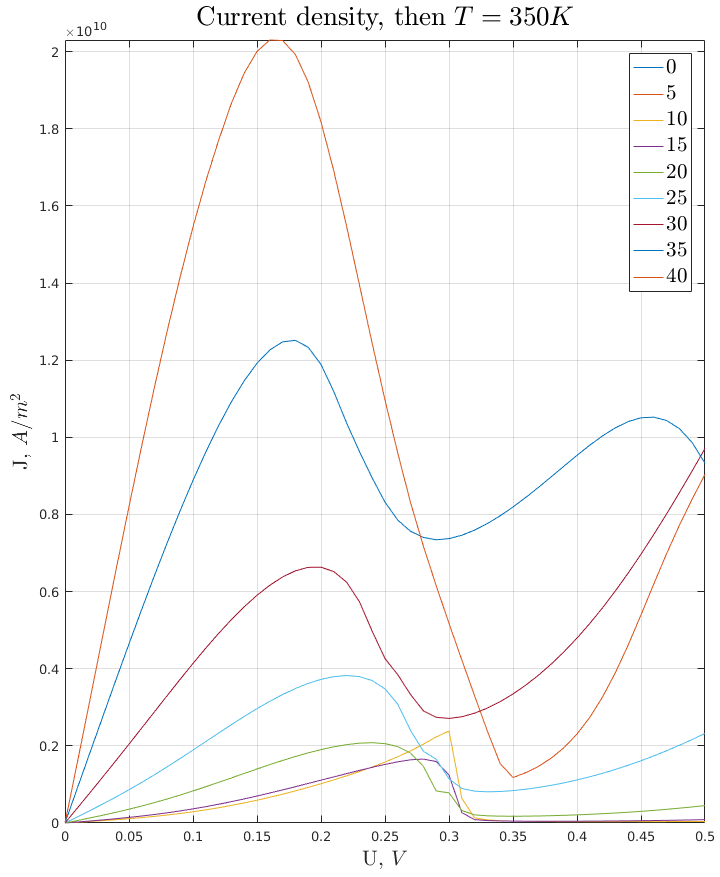
\includegraphics[width=0.38\textwidth]{assets/J1DAlGaAs_Si}

			Система при $T = 350K$ и $Nd = 2*10^{17} sm^{-3}$
		\end{center}
\end{frame}

\end{document}

% \begin{frame}
% 	\frametitle{Цели и задачи}
% \end{frame}

% \begin{columns}
% \column{0.5\textwidth}
% \column{0.5\textwidth}
% \end{columns}